\section*{Novelty Scale}
\begin{description}[noitemsep]
\item[Level 1] Routine design problems solved by methods well known within the specialty - usually 
no invention needed.
\item[Level 2] Minor improvements to an existing system using methods known within the industry.
\item[Level 3] Fundamental improvement to an existing system using methods known outside the 
industry.
\item[Level 4] A new generation of a system that entails a new principle for performing the system's 
primary functions - solutions are found more often in science than technology.
\item[Level 5] A rare scientific discovery or pioneering invention of an essentially new system.
\end{description}

\begin{figure}[H]
\centering
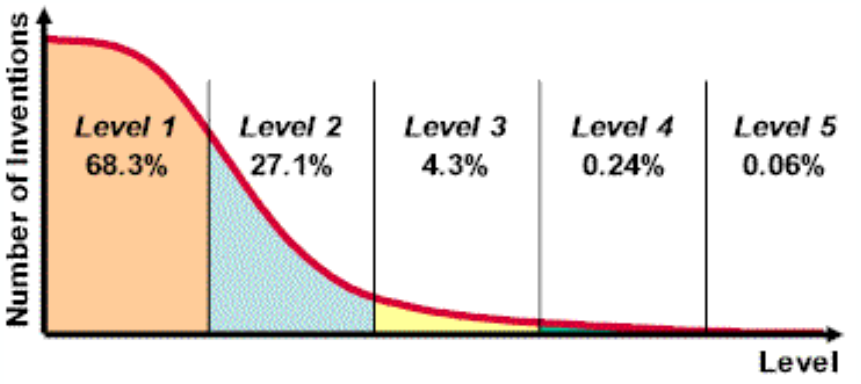
\includegraphics[width=0.7\columnwidth]{Selection_006.png}
\caption{The novelty scale\label{fig:novelty}}
\end{figure}

Based on the nature of our project we have determined that the application is level 2 on the novelty scale. Looking at existing solutions we do not invent any new methods or systems, but we improve on both design and the search algorithm. We do not provide the industry with anything new or innovative, but we make improvements on existing solutions beyond design issues.



%%% Local Variables: 
%%% mode: latex
%%% TeX-master: t
%%% End: 
